\documentclass{article}
\usepackage[utf8]{inputenc}
\usepackage[spanish]{babel}
\usepackage{graphicx}
\usepackage{geometry}
\usepackage{enumerate}
\usepackage{titlesec}
\usepackage{float}
\usepackage{listings}
\usepackage{xcolor}
\usepackage{amsmath}
\usepackage{matlab-prettifier}
\usepackage{amssymb}
\usepackage{tabularx}

\geometry{letterpaper, margin = 1.5cm}

\newcommand{\codefontsize}{\fontsize{10}{11}}
\lstset{
	style = Matlab-editor,
	basicstyle = \codefontsize\ttfamily,
	mlshowsectionrules = true,
	upquote = true,
	tabsize = 4,
	captionpos = b,
	breaklines = true,
	breakatwhitespace = true,
	frame = single,
}

%Datos de la Portada
\title{Introducción a la Programación \ Practica 5}
\author{Medina Martinez Jonathan Jason \ 2023640061}
\date{7 de abril del 2023}

\begin{document}
	
	\fontsize{12}{16}\selectfont
	
	\begin{figure}[t]
		
		
\includegraphics[width=2.5 cm]{Logo1.jpeg}
		\hfill
		
\includegraphics[width=3 cm]{Logo2.png}
		
	\end{figure}
	
	\maketitle
	\newpage
	
	\tableofcontents
	\newpage
	
	\section{Objetivo}
	
	Aplicar las diferentes sentencias de control que permitan resolver problemas.
	
	\section{Introducción}
	
	En esta práctica, se presentan varios problemas que pueden ser resueltos mediante la programación y el uso de estructuras de control, como la estructura condicional if-else y la estructura repetitiva while.
	
	Algunos de los problemas abordados en esta práctica incluyen el cálculo de las raíces reales de una función cuadrática, el cálculo de la suma de los ángulos interiores de una figura geométrica cerrada, la suma de los términos de una serie matemática, el cálculo de la suma de los elementos positivos de un vector y la ordenación de los elementos de un vector en orden descendente utilizando el método de la burbuja.
	
	\newpage
	\section{Desarrollo}
	
	\subsection{Discriminante}
	
	Escriba un programa que calcule las raíces reales de una función cuadrática $ax^2+bx+c = 0$. Cuando el programa se ejecute, este debe pedir al usuario que introduzca los valores de las constantes $a$, $b$ y $c$.
	\newline
	
	Para calcular las raíces de la ecuación, el programa calculará el discriminante $D: D=b^2-4ac$.
	
	\begin{enumerate}[a)]
		\item Si $D > 0$, el programa mostrará un mensaje del tipo: ‘La ecuación tiene dos raíces’, y los valores de las raíces se visualizarán en la línea siguiente.
		
		\item Si $D = 0$, el programa mostrará un mensaje del tipo: ‘La ecuación tiene una raíz’, y el valor de la raíz se visualizará en la línea siguiente.
		
		\item Si $D < 0$, el programa mostrará un mensaje del tipo: ‘La ecuación no tiene raíces reales’.
	\end{enumerate}
	
	\subsubsection{Función}
	
	\begin{lstlisting}
	
	function d = discriminante(a, b, c)
	
	function d = discriminante(a, b, c)
	% DISCRIMINANTE Determina el discriminante de una funcion Ax^2 + Bx + C.
	% Sintaxis:
	% d = discriminante(a, b, c)
	% Entradas:
	% a - El valor de A
	% b - El valor de B
	% c - El valor de C
	% Salida:
	% d - El discriminante.
	
	d = (b^2) - (4*a*c);
	end
	\end{lstlisting}
	
	\subsubsection{Programa1}
	
	\begin{lstlisting}
	
	% Este Programa resuelve ecuaciones de segundo grado de la forma:
	% Ax^2 + Bx + C
	
	A = input('Introduzca el valor de a: ');
	B = input('Introduzca el valor de b: ');
	C = input('Introduzca el valor de c: ');
	
	D = discriminante(A,B,C);
	
	if D > 0
		x1 = ((B*(-1)) + sqrt(D)) / (2*A);
		x2 = ((B*(-1)) - sqrt(D)) / (2*A);
		fprintf('La ecuacion tiene dos raices: x1 = %f y x2 = %f\n', x1, x2);
	elseif D == 0
		x = (B*(-1)) / (2*A);
		fprintf('La ecuacion tiene una raiz: x = %f\n', x);
	else
		fprintf('La ecuacion no tiene raices reales.\n');
	end
	\end{lstlisting}
	
	\subsubsection{Ejecución}
	
	\begin{itemize}
	\item[$\square$] $2x^2+8x-3=0$		
	
	\begin{lstlisting}
	>> Programa1
	Introduzca el valor de a: 2
	Introduzca el valor de b: 8
	Introduzca el valor de c: -3
	La ecuacion tiene dos raices: x1 = 0.345208 y x2 = -4.345208
	\end{lstlisting}
	
	\item[$\square$] $15x^2+10x+5=0$
	
	\begin{lstlisting}
	>> Programa1
	Introduzca el valor de a: 15
	Introduzca el valor de b: 10
	Introduzca el valor de c: 5
	La ecuacion no tiene raices reales.
	\end{lstlisting}
	
	\item[$\square$] $18x^2+12x+2=0$
	
	\begin{lstlisting}
	>> Programa1
	Introduzca el valor de a: 18
	Introduzca el valor de b: 12
	Introduzca el valor de c: 2
	La ecuacion tiene una raiz: x = -0.333333
	\end{lstlisting}
	
	\end{itemize}
	
	\newpage
	
	\subsection{Ángulos}
	
	Con la finalidad de tener una figura geométrica cerrada compuesta de lineas rectas, como se muestra en la siguiente figura, los ángulos en la figura deben sumar: (n-2)(180°) donde n es el numero de lados.
	\\
	
	Pruebe este enunciado usted mismo mediante la creacion de un vector llamado n desde 3 hasta 6 y calcule la suma de angulo a partir de la formula.
	
	\subsubsection{Prueba}
	
	\begin{lstlisting}
	
	>> n = [3:1:6]
	
	n =
	
	3              4              5              6       
	
	>> (n-2)*(180)
	
	ans =
	
	180            360            540            720   
	
	\end{lstlisting}
	
	Escriba un programa que solicite al usuario seleccionar uno de los siguientes:
	
	\begin{itemize}
		\item Triangulo
		\item Cuadrado
		\item Pentágono
		\item Hexágono
	\end{itemize}
	
	Use la entrada para definir el valor de n mediante una estructura \textbf{switch/case}; luego use n para calcular la suma de los ángulos interiores de la figura.
	\\
	
	Modifique su programa de modo que muestre un menú con las opciones del inciso anterior.
	
	\subsubsection{Programa2}
	
	\begin{lstlisting}
		
		%Este programa determina la suma de los angulos internos de un poligono
		%dado.
		
		fprintf('Elija una de las siguientes Poligonos\n');
		
		fprintf('(1) Triangulo\n');
		fprintf('(2) Cuadrado\n');
		fprintf('(3) Pentagono\n');
		fprintf('(4) Hexagono\n');
		
		figura = input('Cual es su Poligono? ');
		
		fprintf('\n');
		
		res = 0;
	\end{lstlisting}
	
	\begin{lstlisting}
		
		switch figura
			case 1
				res = (3-2)*(180);
				fprintf('La suma de los angulos es: %d\n', res);
				
			case 2
				res = (4-2)*(180);
				fprintf('La suma de los angulos es: %d\n', res);
				
			case 3
				res = (5-2)*(180);
				fprintf('La suma de los angulos es: %d\n', res);
				
			case 4
				res = (6-2)*(180);
				fprintf('La suma de los angulos es: %d\n', res);
				
			otherwise
				fprintf('ERROR\n');
				
		end
	\end{lstlisting}
	
	\subsubsection{Ejecución}
	
	\begin{lstlisting}
	
	>> Programa2
	Elija una de las siguientes Poligonos
	(1) Triangulo
	(2) Cuadrado
	(3) Pentagono
	(4) Hexagono
	Cual es su Poligono? 4
	
	La suma de los angulos es: 720
	
	\end{lstlisting}
	
	\begin{lstlisting}
	
	>> Programa2
	Elija una de las siguientes Poligonos
	(1) Triangulo
	(2) Cuadrado
	(3) Pentagono
	(4) Hexagono
	Cual es su Poligono? 1
	
	La suma de los angulos es: 180
	
	\end{lstlisting}
	
	En caso de un dato diferentes a los del menú ocurre lo siguiente:
	\\
	
	\begin{lstlisting}
	
	>> Programa2
	Elija una de las siguientes Poligonos
	(1) Triangulo
	(2) Cuadrado
	(3) Pentagono
	(4) Hexagono
	Cual es su Poligono? 5
	
	ERROR
	
	\end{lstlisting}
	
	\newpage
	
	\subsection{Serie de Leibniz}
	
	Escriba un programa (utilizando un bucle) que calcule la suma de los m primeros términos de la serie:
	
	$$\sum_{n=0}^m \frac{(-1)^n}{2n+1}$$
	
	Esta serie se denomina serie de Leibniz, y converge a $\frac{\pi}{4}$. Ejecute el programa para $m = 10$ y $m = 500$. Compare posteriormente estos resultados con el valor exacto $\frac{\pi}{4}$.
	
	\subsubsection{Programa3}
	
	\begin{lstlisting}
	
	%Este programa permite al usuario ingresar el valor de m de la serie de
	%Leibniz y calcular la suma de sus terminos desde n = 0 hasta el valor de
	%m.
	
	format long;
	
	m = input('Ingrese el valor de m: ');
	
	suma = 0;
	
	for n = 0:m
	suma = suma + (-1)^n / (2*n+1);
	end
	
	disp(['La suma de los primeros ', num2str(n), ' terminos es: ']);
	disp(suma);
	
	pi_cuartos = pi / 4;
	
	disp('el valor de pi/4 es de:');
	disp(pi_cuartos);
	
	\end{lstlisting}
	
	\subsubsection{Ejecución}
	
	m = 10\\
	
	\begin{lstlisting}
	
	>> Programa3
	Ingrese el valor de m: 10
	La suma de los primeros 10 terminos es: 
	0.808078952351398
	
	el valor de pi/4 es de:
	0.785398163397448
	
	\end{lstlisting}
	
	m = 500\\
	
	\begin{lstlisting}
	
	>> Programa3
	Ingrese el valor de m: 500
	La suma de los primeros 500 terminos es: 
	0.785897164896447
	
	el valor de pi/4 es de:
	0.785398163397448
	
	\end{lstlisting}
	\newpage
	
	\subsection{Suma de los elementos de un Vector}
	
	Sea el vector $x = [15, -6, 0, 8, -2, 5, 4, -10, 0.5, 3]$. Escriba un programa que utilice sentencias condicionales y bucles para calcular la suma de los elementos positivos del vector $x$.
	
	\subsubsection{Programa4}
	
	\begin{lstlisting}
	
	%Este Programa solicita al usuario un vector y suma los elementos positivos
	%de dicho vector.
	
	format default;
	
	x = input('Ingrese el vector x: ');
	
	suma = 0;
	
	for i = 1:length(x)
	if x(i) > 0
	suma = suma + x(i);
	end
	end
	
	disp('La suma de los elementos positivos del vector x es: ');
	disp(suma);
	
	\end{lstlisting}
	
	\subsubsection{Ejecución}
	
	Creamos el vector x
	\\
	
	\begin{lstlisting}
	
	>> x = [15, -6, 0, 8, -2, 5, 4, -10, 0.5, 3]
	x =
	Columns 1 through 7
	15.0000   -6.0000         0    8.0000   -2.0000    5.0000    4.0000
	Columns 8 through 10
	-10.0000    0.5000    3.0000
	
	\end{lstlisting}
	 
	 Lo probamos en el programa
	 \\
	 
	 \begin{lstlisting}
	 
	 >> Programa4
	 Ingrese el vector x: x
	 La suma de los elementos positivos del vector x es: 
	 35.5000
	 
	 \end{lstlisting}
	 \newpage
	 
	 \subsection{Burbuja}
	 
	 Escriba una función que ordene los elementos de un vector de cualquier longitud, de mayor a menor utilizando el metido de la burbuja.
	 \\
	 
	 La entrada de la función sera un vector $x$ de cualquier longitud, y la salida sera un vector que contendrá los elementos de $x$ en orden descendente. No se puede utilizar la función predefinida de MATLAB sort para este ejercicio.
	 
	 \subsubsection{Burbuja}
	 
	 \begin{lstlisting}
	 	
	 	function vector = burbuja(x)
	 	
	 	% BURBUJA Esta funcion acomoda un vector en forma descendente a partir de
	 	% un vector dado utilizando el metodo de la burbuja.
	 	%
	 	% vector = burbuja(x)
	 	%
	 	% Entradas:
	 	% x - Vector a acomodar.
	 	% 
	 	% Salida:
	 	% vector - Vector acomodado.
	 	
	 	n = length(x);
	 	
	 	vector = x;
	 	
	 	for i = 1:n-1
		 	for j = 1:n-i
			 	if vector(j) < vector(j+1)
				 	temp = vector(j);
				 	vector(j) = vector(j+1);
				 	vector(j+1) = temp;
			 	end
			end
		end
		
	 	end
	 	
	 \end{lstlisting}
	 
	 Cree su propia función y pruebela con un vector de 14 elementos (enteros) generados aleatoriamente y distribuidos entre -30 y 30.
	 \\
	 
	 Utilice la función rand de MATLAB para generar el vector inicial.
	 
	 \subsubsection{Ejecución}
	 
	 Creamos el vector
	 \\
	 
	\begin{lstlisting}
	
	>> vec = randi([-30,30],1,14)
	
	vec =
	
	Columns 1 through 13
	
	16    18   -19    -1    -3     9    13    16   -14    11     9   -21   -23   0
	
	\end{lstlisting}
	
	Utilizamos el programa para ordenar el vector creado
	\\
	
	\begin{lstlisting}
		
	>> burbuja(vec)
	
	ans =
	
	Columns 1 through 12
	
	18    16    16    13    11     9     9     0    -1    -3   -14   -19  -21   -23
	
	\end{lstlisting}
	\newpage
	
	\subsection{Cartesiano a Polar}
	
	Escriba una función MATLAB que calcule las coordenadas polares de un punto correspondiente a un sistema de coordenadas cartesianas, en un plano de dos dimensiones.\\
	
	Utilice la siguiente línea de definición de función:
	
	\begin{verbatim}
		[theta, radio] = CartesianoAPolar(x, y)
	\end{verbatim}
	
	Los argumentos de entrada serán las coordenadas cartesianas $x$ e $y$ del punto, y los argumentos de salida serán el ángulo $\theta$ y la distancia radial (radio) al punto en cuestión.\\
	
	El ángulo $\theta$ vendrá dado en grados, y su medida será relativa al eje $x$ positivo, de tal forma que sea un número positivo en los cuadrantes I, II y III, y un número negativo en el cuadrante IV.\\
	
	\subsubsection{Función}
	
	\begin{lstlisting}
	
	function res = CartesianoAPolar(x, y)
	
	% CARTESIANOAPOLAR es una funcion que toma las coordenadas cartesianas x e
	% y, devuelve un angulo y una distancia.
	%
	% res = CartesianoAPolar(x, y)
	%
	% Entradas:
	% x - La cordenada x.
	% y - La cordenada y.
	% 
	% Salidas:
	% theta - Es el angulo.
	% radio - La distancia.
	
	radio = hypot(x, y);
	
	theta = atan2d(y, x);
	
	if (theta < 0)
		theta = 360 + theta;
	end
	
	res = [radio, theta];
	
	end
	
	\end{lstlisting}
	
	Utilice posteriormente esta función para calcular las coordenadas polares de los puntos $(15, 3)$, $(-7, 12)$, $(-17, -9)$, $(10, -6.5)$.\\
	
	\subsubsection{Ejecución}
	
	\begin{lstlisting}
	>> CartesianoAPolar(15, 3)
	
	ans =
	
	15.2971   11.3099
	\end{lstlisting}
	
	\begin{lstlisting}
	>> CartesianoAPolar(-7, 12)
	
	ans =
	
	13.8924  120.2564
	\end{lstlisting}
	
	\begin{lstlisting}
	>> CartesianoAPolar(-17, -9)
	
	ans =
	
	19.2354  207.8973
	\end{lstlisting}
	
	\begin{lstlisting}
	>> CartesianoAPolar(10, -6.5)
	
	ans =
	
	11.9269  326.9761
	\end{lstlisting}
	
	\newpage
	
	\subsection{Fibonacci (for)}
	Una secuencia de Fibonacci esta compuesta de elementos creados al sumar los dos elementos previos. La secuencia de Fibonacci mas simples comienza con 1, 1 y procede del modo siguiente: 1, 1, 2, 3, 5, 8, 13, ... Sin embargo, una secuencia de Fibonacci se puede crear con cualesquiera dos números iniciales.
	
	Escriba un programa que solicite al usuario ingresar los dos primeros números en una secuencia de Fibonacci y el numero total de elementos solicitados para la secuencia.
	
	Encuentre la secuencia utilizando un bucle \textbf{for}.
	
	\subsubsection{Programa7}
	
	\begin{lstlisting}
	
	% Este Programa solicita 2 numeros enteros cualesquiera al usuario y una
	% cantidad de elementos de la serie de Fibonacci que se genera con dichos
	% numeros y los imprime en pantalla.
	
	fprintf('\n');
	e1 = input('Ingrese el Primer digito: ');
	fprintf('\n');
	e2 = input('Ingrese el Segundo digito: ');
	fprintf('\n');
	m = input('Ingrese el numero de elementos: ');
	fprintf('\n');
	
	fprintf('%d, ', e1);
	fprintf('%d, ', e2);
	
	for n = 0:m-1
		e3 = e1 + e2;
		fprintf('%d, ', e3);
		e1 = e2;
		e2 = e3;
	end
	
	e3 = e1 + e2;
	
	fprintf('%d\n', e3);
	fprintf('\n');
	
	\end{lstlisting}
	
	\subsubsection{Ejecución}
	
	\begin{lstlisting}
	>> Programa7
	
	Ingrese el Primer digito: 1
	
	Ingrese el Segundo digito: 1
	
	Ingrese el numero de elementos: 10
	
	1, 1, 2, 3, 5, 8, 13, 21, 34, 55, 89, 144, 233
	\end{lstlisting}
	
	\begin{lstlisting}
	>> Programa7
	
	Ingrese el Primer digito: 10
	
	Ingrese el Segundo digito: 25
	
	Ingrese el numero de elementos: 10
	
	10, 25, 35, 60, 95, 155, 250, 405, 655, 1060, 1715, 2775, 4490
	\end{lstlisting}
	
	\newpage
	
	\subsection{Fibonacci (while)}
	
	Repita el problema anterior, esta vez con un bucle \textbf{while}.
	
	\subsubsection{Programa8}
	
	\begin{lstlisting}
	
	% Este Programa solicita 2 numeros enteros cualesquiera al usuario y una
	% cantidad de elementos de la serie de Fibonacci que se genera con dichos
	% numeros y los imprime en pantalla.
	
	fprintf('\n');
	
	e1 = input('Ingrese el Primer digito: ');
	fprintf('\n');
	
	e2 = input('Ingrese el Segundo digito: ');
	fprintf('\n');
	
	m = input('Ingrese el numero de elementos: ');
	fprintf('\n');
	
	fprintf('%d, ', e1);
	
	fprintf('%d, ', e2);
	
	n = 0;
	
	while n < m-1
		e3 = e1 + e2;
		fprintf('%d, ', e3);
		e1 = e2;
		e2 = e3;
		n = n +1;
	end
	
	e3 = e1 + e2;
	
	fprintf('%d\n', e3);
	fprintf('\n');
	
	\end{lstlisting}
	
	\subsubsection{Ejecución}
	
	\begin{lstlisting}
	>> Programa8
	
	Ingrese el Primer digito: 1
	
	Ingrese el Segundo digito: 1
	
	Ingrese el numero de elementos: 10
	
	1, 1, 2, 3, 5, 8, 13, 21, 34, 55, 89, 144
	
	\end{lstlisting}
	
	\begin{lstlisting}
	>> Programa8
	
	Ingrese el Primer digito: 12
	
	Ingrese el Segundo digito: 25
	
	Ingrese el numero de elementos: 12
	
	12, 25, 37, 62, 99, 161, 260, 421, 681, 1102, 1783, 2885, 4668, 7553
	
	\end{lstlisting}
	
	\newpage
	
	\subsection{Numero Áureo}
	
	Una propiedad interesante de una secuencia de Fibonacci es que la razón de los valores de miembros adyacentes de la secuencia se aproxima a un numero llamado “numero áureo” o $\Phi$ (Phi).
	\\
	
	El valor numérico de $\Phi$, representado mediante radicales o decimales es:
	
	\begin{equation*}
	\Phi = \frac{1 + \sqrt{5}}{2} = 1.618033988749894 \dots
	\end{equation*}
	
	Por ejemplo, si tomamos dos números naturales arbitrarios, por ejemplo 5 y 6, la secuencia de Fibonacci resulta: 5, 6, 11, 17, 28, 45, 73, 118, 191, 309, $\ldots$.
	\\
	
	Los cocientes de términos sucesivos producen aproximaciones racionales que se acercan asintóticamente por exceso y por defecto al mismo límite, es decir, si calculamos el cociente de los números 17 y 28 de la secuencia anterior, que son números consecutivos, obtenemos $28/17 = 1.64705882 \ldots$; si repetimos el proceso con los siguientes pares de valores de la sucesión notamos lo siguiente: $45/28 = 1.60714285 \ldots$; $73/45 = 1.622222222 \ldots$; $118/73 = 1.616438356 \ldots$; $191/118 = 1.61864406 \ldots$; $309/191 = 1.617801047 \ldots$, y así sucesivamente.
	\\
	
	Cree un programa que acepte los primeros dos números de una secuencia de Fibonacci como entrada de usuario y luego calcule valores adicionales en la secuencia hasta que la diferencia entre las razones de valores adyacentes sea de 0.001.
	\\
	
	Puede hacer esto con un bucle while al comparar la razón del elemento $k$ con el elemento $k-1$ y la razón del elemento $k-1$ con el elemento $k-2$. Si llama a su secuencia fib, entonces la sentencia while sería algo como:
	
	\begin{equation*}
		\text{while} \left|\frac{\text{fib}(k)}{\text{fib}(k - 1)} - \frac{\text{fib}(k - 1)}{\text{fib}(k - 2)}\right| > 0.001
	\end{equation*}
	
	Una vez obtenidos los valores, cree una gráfica donde muestre los cocientes de los valores adyacentes de la sucesión calculada.
	
	\newpage
	
	\subsubsection{Programa9}
	
	\begin{lstlisting}
	
	% Programa que solicita los primeros dos numeros de una secuencia de
	% Fibonacci como entrada de usuario y luego calcule valores adicionales en 
	% la secuencia hasta quela diferencia entre las razones de valores 
	% adyacentes sea de 0.001 y crea una grafica de los cocientes de los 
	% valores adyacentes de la sucesion calculada.
	
	format long;
	
	phi = (1 + sqrt(5))/2;
	
	fprintf('\n')
	
	e1 = input('Ingrese el Primer digito: ');
	fprintf('\n');
	
	e2 = input('Ingrese el Segundo digito: ');
	fprintf('\n');
	
	e3 = 0;
	rac = 0;
	vec = [e2/e1];
	
	fprintf('%d, ', e1);
	
	fprintf('%d, ', e2);
	
	while abs(rac - phi) >= 0.001
		rac = abs(e2 / e1);
		vec = [vec, rac];
		e3 = e1 + e2;
		fprintf('%d, ', e3);
		e1 = e2;
		e2 = e3;
	end
	
	fprintf('\n\n');
	
	fprintf('El valor de Phi es: %f', phi);
	
	fprintf('\n\n');
	
	fprintf('El valor de %d / %d es: %f', e2, e1, phi);
	
	fprintf('\n\n');
	
	
	plot(vec);
	title('Cocientes de valores adyacentes en la secuencia de Fibonacci');
	
	\end{lstlisting}
	
	\newpage
	
	\subsubsection{Ejecución}
	
	\begin{lstlisting}
	
	>> Programa9
	
	Ingrese el Primer digito: 5
	
	Ingrese el Segundo digito: 6
	
	5, 6, 11, 17, 28, 45, 73, 118, 191, 309, 
	
	El valor de Phi es: 1.618
	
	El valor de 309 / 191 es: 1.618
	
	\end{lstlisting}
	
	\subsubsection{Grafica}
	
	\begin{figure*}[h]
		\centering
		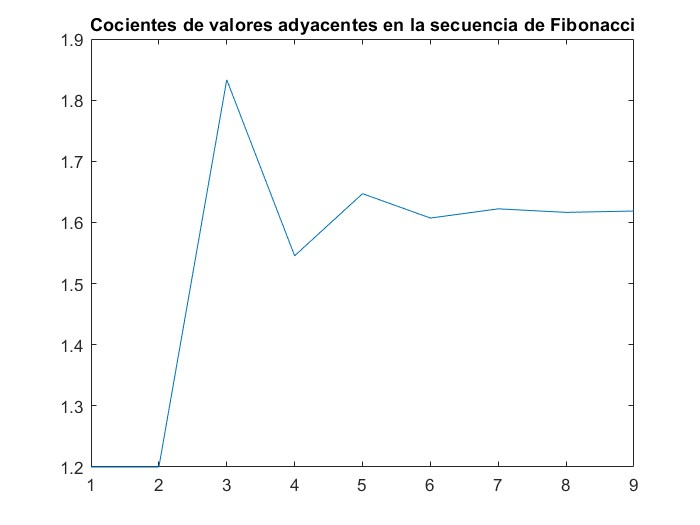
\includegraphics[width=\textwidth]{Grafica9.jpg}
	\end{figure*}
	
	\newpage
	
	\subsection{For}
	
	Siempre que sea posible, es mejor evitar el uso de bucles for, puesto que son lentos para ejecutar. Para comprobar esto:
	
	\begin{enumerate}[a)]
	\item Genere un vector de $100,000,000$ valores aleatorios llamado $x$; eleve al cuadrado cada elemento en este vector, utilizando una operación elemento a elemento, y asigne el resultado a $y$; use los comandos \textbf{tic} y \textbf{toc} para cronometrar la operación.
	
	\subsubsection{Programa10a}
	
	\begin{lstlisting}
		
	% Programa que genera un vector x de numeros pseudo-aleatorios de 1 a 
	% 100000000 y luego eleva al cuadrado cada elemento de dicho vector
	% asignandolo a el vector y y cronometra el tiempo que tarda en realizar
	% dicha operacion imprimiendo dicho tiempo en pantalla
	
	tic
	x = rand(1,100000000);
	
	y = x.^2;
	toc
	
	\end{lstlisting}
	
	\subsubsection{Ejecución}
	
	\begin{lstlisting}
	>> Programa10a
	Elapsed time is 0.646970 seconds.
	
	\end{lstlisting}
	
	\item A continuación, realice la misma operación utilizando un bucle \textbf{for}. Antes de comenzar, limpie los valores en sus variables con el comando \textbf{clear x y}
	Use los comandos \textbf{tic} y \textbf{toc} para cronometrar la operación.
	
	\subsubsection{Programa10b}
	
	\begin{lstlisting}
		
	% Este Programa realiza lo mismo que el Programa10a.m solo que ahora
	% realiza un la operacion de elevar los elementos del vector x y asignarlos
	% en el vector y con un ciclo for.
	
	clear x y;
	
	tic
	x = rand(1,100000000);
	
	for i=1:length(x)
		y(i) = x(i)^2;
	end
	toc
	
	\end{lstlisting}
	
	\subsubsection{Ejecución}
	
	\begin{lstlisting}
	>> Programa10b
	Elapsed time is 5.556869 seconds.
	\end{lstlisting}
	
	\item Si va a usar un valor constante muchas veces dentro de un bucle \textbf{for}, calculelo, una vez y almacenelo en una variable, en lugar de calcularlo cada vez en el bucle. Para demostrar esto, cree un bucle \textbf{for} que vaya desde 1 hasta 10,000,000 en incrementos de 1, que sirva para inicializar un vector x con el valor
	\begin{equation*}
		(\sin(0.3) + \cos(\frac{\pi}{3})) * 5!
	\end{equation*}
	
	Primero, asegúrese de hacer la operación dentro del bucle \textbf{for} y tome el tiempo que tarda la operación. Posteriormente, cree una variable fuera del bucle \textbf{for} donde asigne el resultado de la operación y utilice dicha variable dentro de su bucle. De igual forma, tome el tiempo que tarda la operación.
	
	\subsubsection{Programa10c}
	
	\begin{lstlisting}
	
	% Programa que toma el tiempo de dos ciclos diferentes uno que inicializa
	% una constante fuera del ciclo for y el otro que no lo inicializa si no 
	% que cada vez que el ciclo se ejecuta cada vez que el ciclo for realiza la
	% operacion.
	
	tic
	
	for i = 1:10000000
		x(i) = (sin(0.3) + cos(pi/3)) * factorial(5);
	end
	
	toc
	
	tic
	
	constant = (sin(0.3) + cos(pi/3)) * factorial(5);
	
	for i = 1:10000000
		x(i) = constant;
	end
	
	toc
	
	\end{lstlisting}
	
	\subsubsection{Ejecución}
	
	\begin{lstlisting}
		
	>> Programa10c
	Elapsed time is 6.105748 seconds.
	Elapsed time is 0.010562 seconds.
	
	\end{lstlisting}
	
	\item Si MATLAB debe aumentar el tamaño de un vector cada vez en un bucle, el proceso tomara mas tiempo que si el vector ya tuviese el tamaño adecuado. Demuestre este hecho al repetir el inciso b) de este ejercicio.
	
	Cree el siguiente vector de valores y, en el que cada elemento sea igual a cero antes de ingresar el bucle for:
	\begin{align*}
		\centering
		\textbf{y = zeros(1,100000000)};
	\end{align*}
	
	 Tome el tiempo que tarda la ejecución y anote sus comentarios y conclusiones.
	 
	 \subsubsection{Programa10d}
	 
	 \begin{lstlisting}
	 
	 tic
	 
	 x = rand(1,100000000);
	 
	 for i=1:length(x)
		 y(i) = x(i)^2;
	 end
	 
	 toc
	 
	 clear x y;
	 
	 tic
	 
	 x = rand(1,100000000);
	 
	 y = zeros(1,100000000);
	 
	 for i=1:length(x)
	 	y(i) = x(i)^2;
	 end
	 
	 toc
	 
	 \end{lstlisting}
 	
 	\subsubsection{Ejecución}
 	
 	\begin{lstlisting}
 	>> Programa10d
 	Elapsed time is 5.659559 seconds.
 	Elapsed time is 0.687611 seconds.
 	\end{lstlisting}
	 
	\end{enumerate}
	
	\newpage
	\section{Conclusión}
	
	En conclusión, la práctica proporciona una oportunidad para aplicar los conceptos aprendidos en las sentencias de control y funciones de MATLAB para resolver problemas matemáticos.
	\\
	
	El declarar las variables, los vectores, etc fuera del ciclo aumenta la velocidad en la que el ciclo for se ejecuta puesto que ya no tiene que recalcular dichas variables o vectores cada ves que se ejecuta.
	
\end{document}